
\section{Bounding Bin Configurations Using Stars and Bars}
\label{app:bounded-config}

\begin{lemma}
\label{lem:bounded-config}
    For any Bin Packing instance with $m$ distinct
    item sizes, each at least $\varepsilon>0$,
    the number of non-empty feasible bin configurations
    $q$ satisfies
    \[
        q\leq \binom{k+m}{m}-1,
        \qquad k=\lfloor 1/\varepsilon\rfloor.
    \]
\end{lemma}

\begin{proof}
Let $c_j$ denote the number of items of size
$y_j$ in a configuration. Since each bin has unit
capacity and every item has size at least $\varepsilon$,
it contains at most $k$ items. Thus,
\[
    \sum_{j=1}^{m}c_j\leq k,
    \qquad c_j\in\mathbb{Z}_{\geq 0}.
\]
Introducing a non-negative integer slack variable
$c_R$ gives the equation
\[
    c_1+c_2+\cdots+c_m+c_R=k,
\]
where all variables are non-negative integers.

This can be interpreted as distributing $k$
identical balls among $m+1$ distinguishable
bins. The first $m$ bins represent the distinct
item sizes, while the last bin represents
unused item slots.

Equivalently, we arrange $k$ identical balls
and $m$ dividers in a row. Each arrangement
uniquely determines a non-negative integer
solution to the equation.

\begin{figure}[htbp]
    \centering
    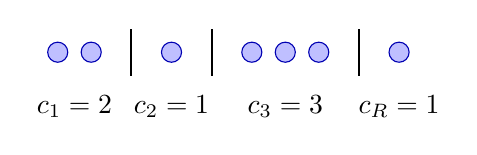
\begin{tikzpicture}[scale=0.85]

        % Seven identical balls
        \foreach \x in {0,0.5,1.7,2.9,3.4,3.9,5.1} {
            \filldraw[fill=blue!25, draw=blue!70!black]
                (\x,0) circle (0.15);
        }

        % Three dividers
        \foreach \x in {1.1,2.3,4.5} {
            \draw[thick] (\x,-0.35) -- (\x,0.35);
        }

        % Labels for each category
        \node[below] at (0.25,-0.5) {$c_1=2$};
        \node[below] at (1.7,-0.5) {$c_2=1$};
        \node[below] at (3.4,-0.5) {$c_3=3$};
        \node[below] at (5.1,-0.5) {$c_R=1$};

    \end{tikzpicture}
    \caption{Stars-and-bars representation with
    $k=7$ balls and $m=3$ dividers.}
    \label{fig:stars-bars}
\end{figure}

As illustrated in \Cref{fig:stars-bars},
each arrangement corresponds to a possible
configuration of item counts.

There are $k+m$ positions, from which we
choose $m$ positions for the dividers.
Hence, the number of arrangements is
\[
    \binom{k+m}{m}.
\]

Exactly one arrangement corresponds to the empty
configuration, with $c_1=\cdots=c_m=0$ and $c_R=k$.
Excluding it leaves $\binom{k+m}{m}-1$ possible
non-empty item-count vectors. Some of these may
violate the bin-capacity constraint or require more
items of a given size than are available. Every feasible
configuration is nevertheless counted, so
$q\leq\binom{k+m}{m}-1$.
\end{proof}
